\documentclass[nosolution]{exercice}
\usepackage[french]{babel}
\usepackage{fancybox}
\usepackage{rotating}
\usepackage{float}
\usepackage[utf8]{inputenc}
\usepackage{fancyhdr}
\usepackage{datetime}
\usepackage{url}

\renewcommand{\dateseparator}{.}
\newcommand{\todayiso}{\twodigit\day \dateseparator \twodigit\month \dateseparator \the\year}

\fancyhead{}
\renewcommand{\headrulewidth}{0pt}
\rfoot{\todayiso}
\pagestyle{fancy}

\graphicspath{{./Images/}}

\newcommand{\includeschema}[1]{\begin{center}\Ovalbox{\includegraphics{#1}}\end{center}}

\newenvironment{portlist}{\begin{center}\begin{tabular}{|c|c|c|l|}\toprule\textbf{Port} & \textbf{Direction} & \textbf{Size} & \textbf{Description} \\\midrule\hline }{\end{tabular}\end{center}}

\newcommand{\oneport}[4]{\texttt{#1} & #2 & $#3$ & #4 \\ \hline}
\newcommand{\lastport}[4]{\texttt{#1} & #2 & $#3$ & #4 \\ \hline}

\floatstyle{ruled}
\newfloat{program}{thp}{lop}
\floatname{program}{Program}

\begin{document}

\noindent
\begin{minipage}[l]{\linewidth}
  \rule{\linewidth}{0.2mm} \\

  {\vspace{-5mm}
    \parpic[r]{\includegraphics[width=4cm]{images/HESSO_logo}}
    \parpic(5cm,4cm)(6.5cm,1.6cm){
\includegraphics[width=5cm]{images/HEIG-VD_logo_couleur_format_JPG.jpg}}
    \hspace{-14mm}{\includegraphics[width=6cm]{images/HEPIA_logo}}\vspace{15mm} \\
    \textbf{Laboratoire de systèmes numériques / Architecture des ordinateurs} \\
    Auteurs: A. Lescourt, Prof. F. Vannel, Prof. A. Upegui (Hepia)\\
    Modifications : Y.Saugy, S.Krieg, A.Convers (HEIG-VD). v.1.2
    }

    \vspace{7mm}

  \begin{center}
    {\Large\textbf{Introduction à l'utilisation de Logisim} \\
      \vspace{5mm}}
  \end{center}

  \rule{\linewidth}{0.2mm}
\end{minipage}


\setlength{\parskip}{5pt}
\setlength{\parsep}{5pt}
\setlength{\topsep}{5pt}
\setlength{\itemsep}{5pt}

\renewcommand{\labelitemi}{$\bullet$}
\renewcommand{\labelitemii}{$-$}
\renewcommand{\labelitemiii}{$\diamond$}
\renewcommand{\labelitemiv}{$\ast$}

%%%%%%%%%%%%%%%%%%%%%%%%
%%%% DEBUT DOCUMENT %%%%
%%%%%%%%%%%%%%%%%%%%%%%%

\section{Introduction}
\texttt{Logisim} est un logiciel open-source permettant de concevoir et de simuler des circuits
logiques~\footnote{La dernière version de Logisim peut être téléchargée à l'adresse
  \url{http://reds-data.heig-vd.ch/logisim-evolution/logisim-evolution.t.jar}.
  Logisim contient un mécanisme d'auto-update: dès qu'une nouvelle version sort, vous recevrez
  une notification au démarrage du logiciel et vous aurez
  la possibilité de le mettre à jour.}.

Ce document est un
tutoriel qui décrit comment établir un système numérique à l'aide de cet éditeur de schéma. Nous expliquerons les
démarches nécessaires afin de concevoir, simuler et implémenter un projet sur une carte \texttt{Altera MAX\_V}.

Il existe différentes façons de décrire formellement les systèmes numériques : des langages de description du matériel
(HDL), des tables de vérité, des graphes d'états, ou des schémas. Logisim permet uniquement de travailler sur des
schémas. Le premier chapitre expliquera comment réaliser un premier schéma.
Vous pouvez voir l'interface de Logisim sur la Figure  \ref{fig_logisim_description}.

\begin{figure}[H]
\begin{center}
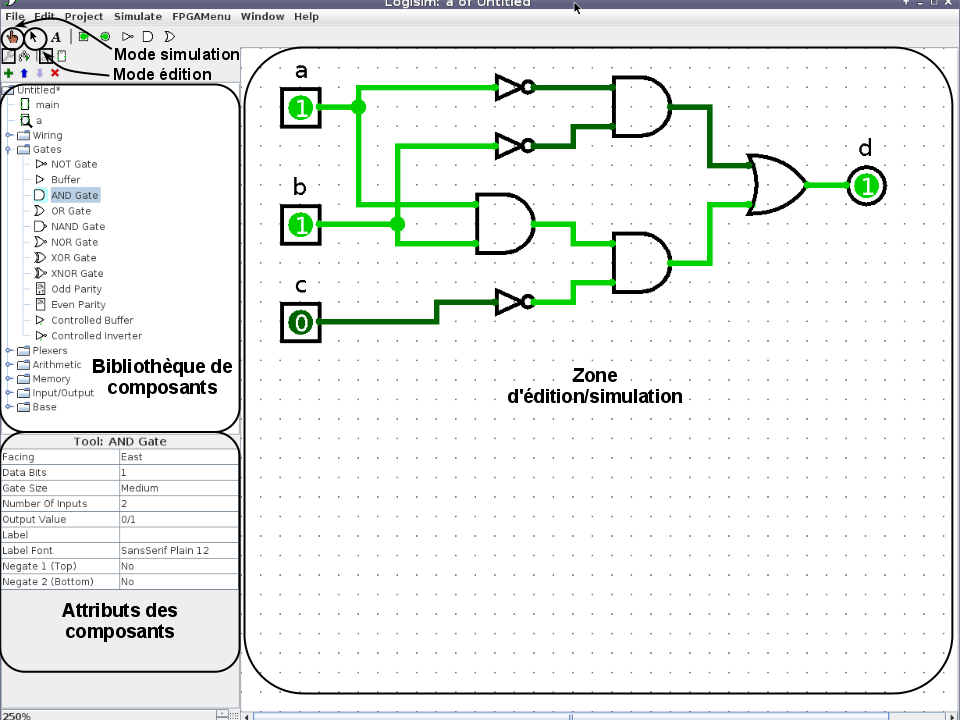
\includegraphics[width=300pt]{images/Logisim_description.png}
\caption{\label{fig_logisim_description}Interface de Logisim}
\end{center}
\end{figure}

Une des particularités de \texttt{Logisim} est de pouvoir éditer et simuler un circuit en même temps.
Nous expliquerons plus tard dans ce document comment simuler un circuit, puis comment l'implémenter sur la carte du
laboratoire.

A l'ouverture de \texttt{Logisim}, une fenêtre demande l'introduction du nom d'utilisateur -- voir Figure \ref{fig_logisim_login}.
Il sera inscrit dans chaque composant créé, afin d'empêcher le plagiat.

\begin{figure}[H]
\begin{center}
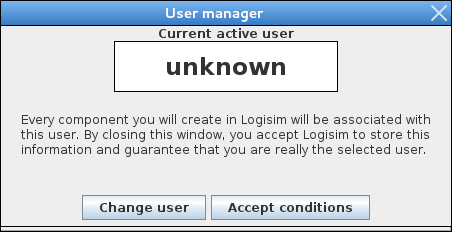
\includegraphics[width=180pt]{images/login.png}
\caption{\label{fig_logisim_login}Fenêtre de login}
\end{center}
\end{figure}

Lors de la première utilisation, il faut ajouter un utilisateur comme en Figure~\ref{fig_logisim_adduser}:
\begin{enumerate}
\item Cliquer sur \texttt{Change user}.

\item Introduire votre prénom et votre nom dans la case \texttt{Add new user}, sous la même forme que votre login Heig-vd, sans caractères spéciaux, séparé par un  \_.

\item Cliquer sur \texttt{Add}.

\item Cliquer sur \texttt{Close}.

\item Cliquer sur \texttt{Accept conditions}.

\end{enumerate}


\begin{figure}[H]
\begin{center}
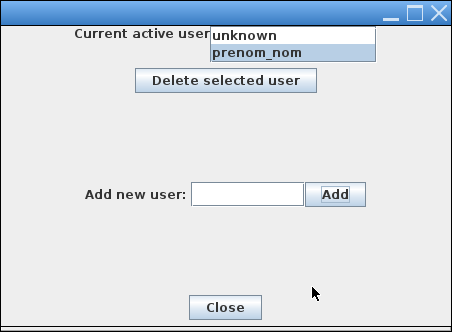
\includegraphics[width=180pt]{images/add_user.png}
\caption{\label{fig_logisim_adduser}Ajout d'un utilisateur}
\end{center}
\end{figure}

La liste des utilisateurs est enregistrée sur la machine. Pour les utilisations ultérieures, il suffit de cliquer sur \texttt{Accept conditions} pour sélectionner l'utilisateur actif ou de le sélectionner dans la liste.

%%%%%%%%%%%%%%%%%%%%%%%%%%%%%%%%%%%%%%%%%%%%%%%%%
\section{Mode édition}
\begin{enumerate}
\item Pour utiliser le mode édition, il faut simplement sélectionner la flèche comme indiqué en haut de la figure
\ref{fig_logisim_description}.
\item On peut alors choisir un composant dans la bibliothèque sur la gauche. Pour l'ajouter dans son schéma, il suffit
de cliquer sur le composant désiré, puis de cliquer sur le schéma.

\item Chaque composant que vous utiliserez aura des attributs modifiables dans la zone inférieur gauche de
\texttt{Logisim}. Par exemple si l'on pose une porte \texttt{AND}, on peut modifier le nombre de signaux qu'elle prend en
entrée, ou encore mettre un inverseur sur une de ses entrées.

\item Il est aussi possible de faire des copier/coller d'un ou plusieurs composants. Dans ce cas, les composants
conserverons aussi tous les attributs préalablement définis.

\item Voici un descriptif des éléments que vous aller avoir besoin pour ce tutorial:
\begin{itemize}
\item Pour les entrées, l'élément \texttt{Pin} de \texttt{Wiring}.
\item Pour les sorties, l'élément \texttt{Pin} de \texttt{Wiring} avec l'attribut \texttt{output?=yes}.
\item Les portes logiques sont présentent dans le répertoire \texttt{Gates}.
\item Le \texttt{splitter} de \texttt{Wiring}.
\item Le \texttt{ground} et \texttt{power} de \texttt{Wiring}.
\end{itemize}

\item Une fois que l'on a posé tous les composants, il faut alors les connecter. Pour cela il suffit de placer le curseur
avec la souris sur un des ports à connecter et, en gardant pressé le bouton
gauche de la souris, le déplacer jusqu'au port de destination.

\end{enumerate}

%%%%%%%%%%%%%%%%%%%%%%%%%%%%%%%%%%%%%%%%%%%%%%%%%
\section{Création d'un premier circuit}



\label{nouveauCircuit}
Tous les circuits réalisés dans \texttt{Logisim} peuvent être réutilisés dans d'autres circuits.
Afin de créer un nouveau circuit, il faut aller dans \texttt{Project} -> \texttt{Add circuit...} -> nommer le circuit. Le circuit créé devient un composant disponible dans la bibliothèque.

\subsection{Add1bit}
Réalisez le schéma en Figure~\ref{fig_logisim_addOneBit}. Nommez le \texttt{Add1bit}.
Remarques:
\begin{itemize}
\item Le circuit en cours d'édition est celui qui comporte une petite loupe en dessous du nom du projet.
\item Ne prenez pas en compte la couleur des fils ni la valeur des \texttt{Pin} d'entrées (ces dernières sont un X bleu par défaut).
\item Vous pouvez changer l'orientation des composants en modifiant l'attribut \texttt{Facing}.
\end{itemize}

\begin{figure}[H]
\begin{center}
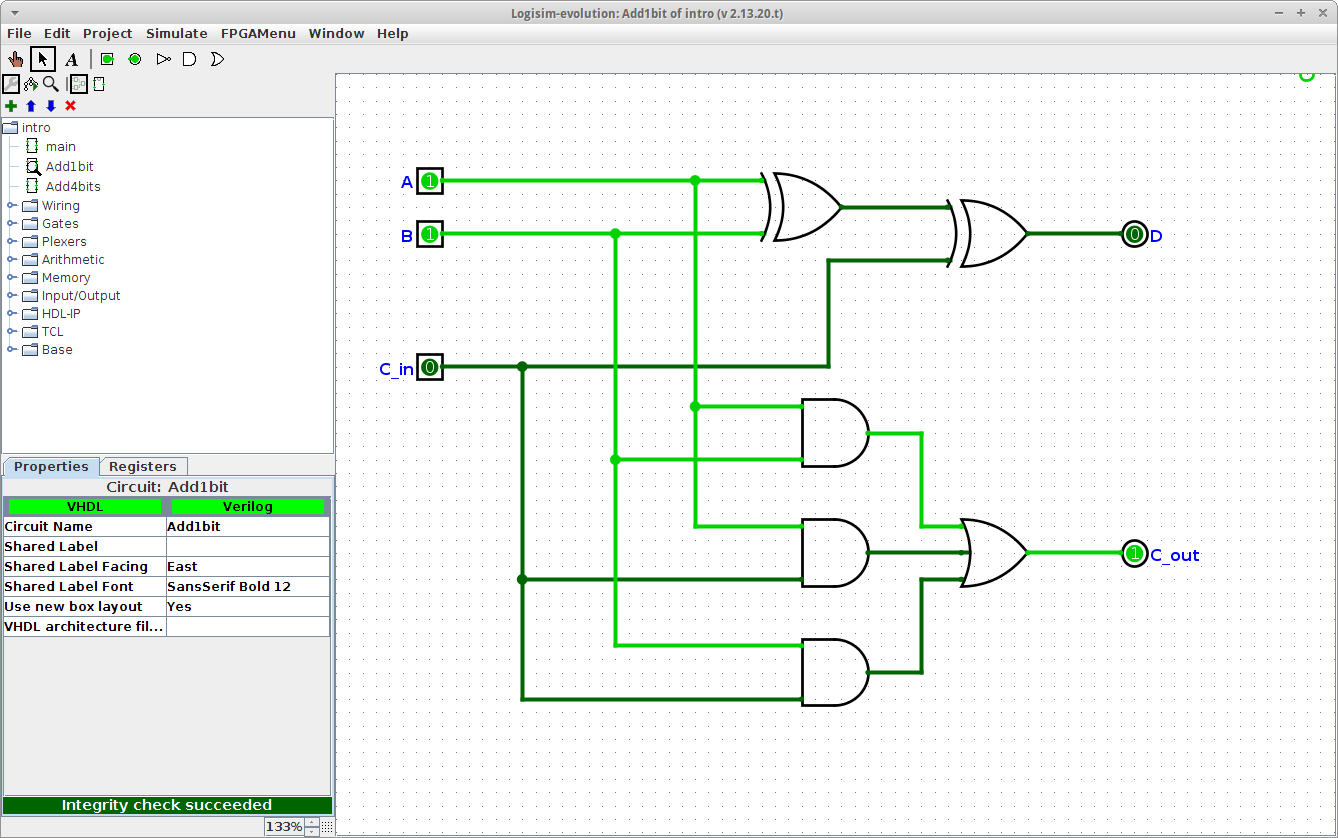
\includegraphics[width=400pt]{images/logisim_add1bit.png}
\caption{\label{fig_logisim_addOneBit}Additionneur 1 bit}
\end{center}
\end{figure}

%%%%%%%%%%%%%%%%%%%%%%%%%%%%%%%%%%%%%%%%%%%%%%%%%
\section{Mode simulation}
\texttt{Logisim} est capable de simuler le circuit en affichant les valeurs des signaux directement sur le schéma. L'utilisateur
peut alors définir les valeurs des bits en entrée et observer la réaction du design.
\begin{enumerate}
\item Pour utiliser le mode simulation, il faut sélectionner la main en haut à gauche de \texttt{Logisim} (cf
Figure~\ref{fig_logisim_description})

\item Il est alors possible de contrôler l'état des différentes entrées en cliquant directement dessus. Le X bleu des
\texttt{Pin} d'entrées représente l'état haute impédance.
Dans ce laboratoire, nous travaillerons uniquement avec des états haut ou bas. Pour supprimer cet état de haute
impédance, il faut modifier les attributs de ces \texttt{Pin} d'entrées de façon à ce que la ligne \texttt{Three-state)}
soit égale à \texttt{No}.

\item En cliquant sur une entrée, la valeur doit alterner entre \texttt{'0'} ou \texttt{'1'}.

\item Voici un descriptif des couleurs utilisées pour les signaux en mode simulation.
\begin{figure}[H]
\begin{center}
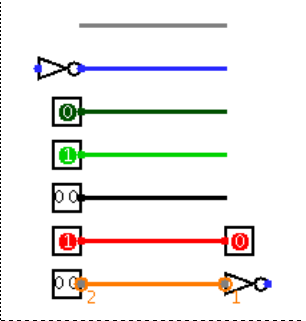
\includegraphics[scale=0.4]{images/logisim_couleurs.png}
\caption{\label{fig_logisim_couleur}Couleurs des fils en simulation}
\end{center}
\end{figure}

\begin{itemize}
\item \textbf{Gris}: La taille du fil est inconnue. Le fil n'est relié à aucune entrée ou sortie.
\item \textbf{Bleu}: Le fil comporte une valeur, cependant elle est inconnue.
\item \textbf{Vert foncé}: Le fil comporte la valeur \texttt{'0'}.
\item \textbf{Vert clair}: Le fil comporte la valeur \texttt{'1'}.
\item \textbf{Noir}: Le fil comporte plusieurs bits (BUS).
\item \textbf{Rouge}: Le fil comporte une erreur.
\item \textbf{Orange}: Les composants reliés au fil n'ont pas la bonne taille.
\end{itemize}

\item Testez le bon fonctionnement de votre additionneur 1 bit.

\end{enumerate}

%%%%%%%%%%%%%%%%%%%%%%%%%%%%%%%%%%%%%%%%%%%%%%%%%
\section{Design hiérarchique}
La méthodologie de design que l'on vient d'utiliser est valable pour la conception de systèmes numériques plutôt
simples, c'est-à-dire avec un nombre de portes logiques plutôt bas. Lorsque l'on vise des systèmes plus compliqués on
risque de voir le nombre de portes et de connexions exploser. Dans ce cas, le risque d'introduire des erreurs devient
très important.

La clé pour gérer correctement une complexité plus grande est d'utiliser le design hiérarchique. Grâce au design
hiérarchique on peut travailler à différents niveaux d'abstraction. D'abord on décrit des blocs de base à l'aide des
portes logiques, pour ensuite utiliser ces blocs de base comme parties d'un système plus large. Dans le cas de notre
additionneur 1 bit, on va en utiliser quatre pour construire un additionneur 4 bits. Ce nouveau bloc pourrait ensuite
faire lui aussi partie d'un autre système plus grand.

Pour créer un design hiérarchique en incluant l'additionneur 1 bit que l'on a déjà conçu, il faudra suivre les pas
suivants:
\begin{enumerate}
\item Créez un nouveau circuit comme déjà expliqué dans la section \ref{nouveauCircuit} et nommez le \texttt{Add4bits}.
Pour passer de l'édition d'un circuit à l'autre, il suffit de double-cliquer sur le nom de celui désiré dans le menu de
gauche.
\item Il est alors possible d'ajouter un sous circuit \texttt{add1bit} de la même manière que l'utilisation d'un
composant quelconque. On clique sur \texttt{Add1bit} dans le menu indiqué sur la Figure~\ref{fig_sousCircuit}, puis on le
place en cliquant sur le circuit.
\item Si le circuit \texttt{Add1Bit} a été créé correctement, alors il devrait être représenté par un petit bloc, avec
sur sa gauche trois points bleus correspondant aux entrées et deux points verts sur sa droite correspondant aux sorties.

\begin{figure}[H]
\begin{center}
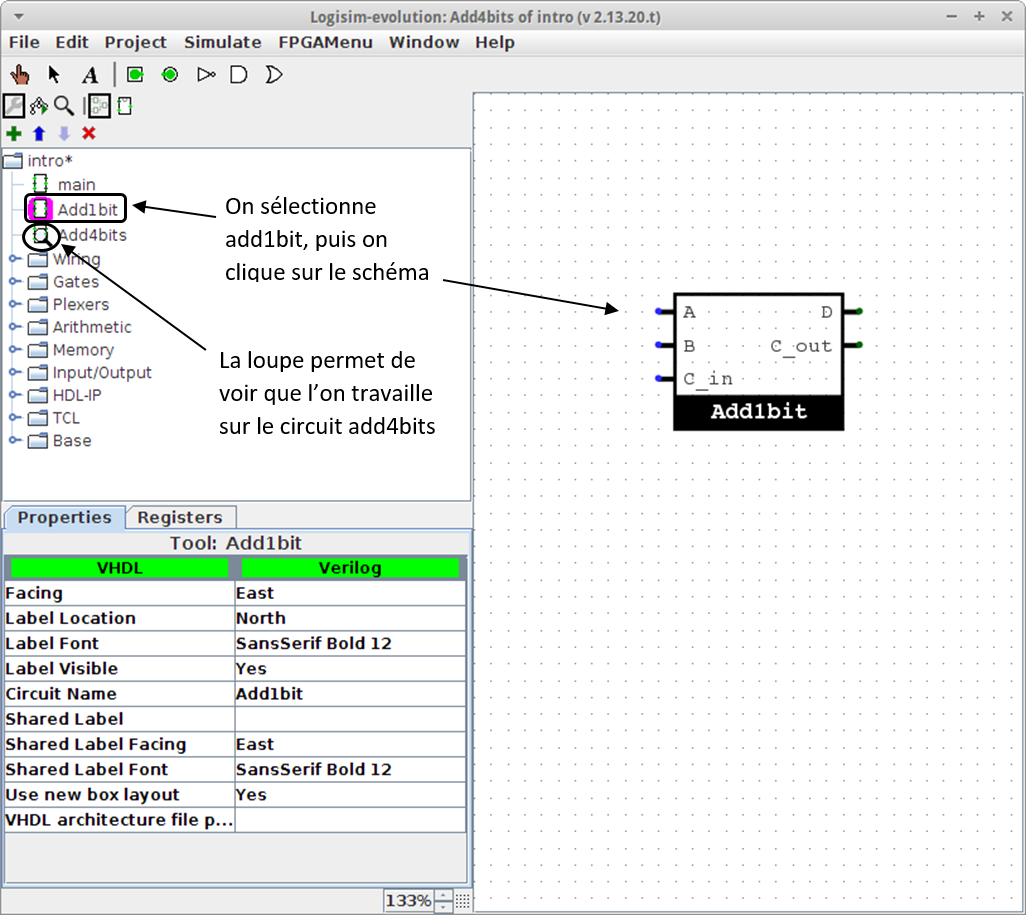
\includegraphics[width=300pt]{images/logisim_sousCircuit.png}
\caption{\label{fig_sousCircuit}Sous circuit}
\end{center}
\end{figure}

\item Si les sorties apparaissent en bleu et non en vert sur le schéma, vérifiez que vous avez bien affecté l'attribut
\texttt{output?=yes} dans les \texttt{pins} de sorties.

\item Pour l'implémentation de l'additionneur 4 bits, il vous faut 4 additionneurs 1 bit, donc complétez le schéma en
incluant les ports d'entrée et sortie. Une des différences entre les circuits pour les additionneurs 1 et 4 bits, est le
fait que dans le premier cas les entrées et sorties étaient toutes des fils indépendants, tandis que dans le deuxième
cas, on a des bus de données à l'entrée et à la sortie. Par exemple, pour définir l'entrée A comme un bus de 4 bits, il
faut ajouter un élément \texttt{pin} et définir sa taille via l'attribut \texttt{Data bits = 4}.

\item Lorsque l'on tire un fil de l'une de ces entrées, ce n'est plus un simple signal mais un bus de 4 bits. Pour
pouvoir connecter les éléments de ce bus aux entrées des additionneurs 1 bits, on va devoir séparer les différents fils
du bus afin de pouvoir les traiter un par un. L'élément \texttt{splitter} de \texttt{wiring} permet d'effectuer ces
conversions dans les deux sens: d'un bus de 4 bits vers 4 fils, et de 4 fils vers un bus de 4 bits --
voir Figure~\ref{fig_splitter}.

\begin{figure}[H]
\begin{center}
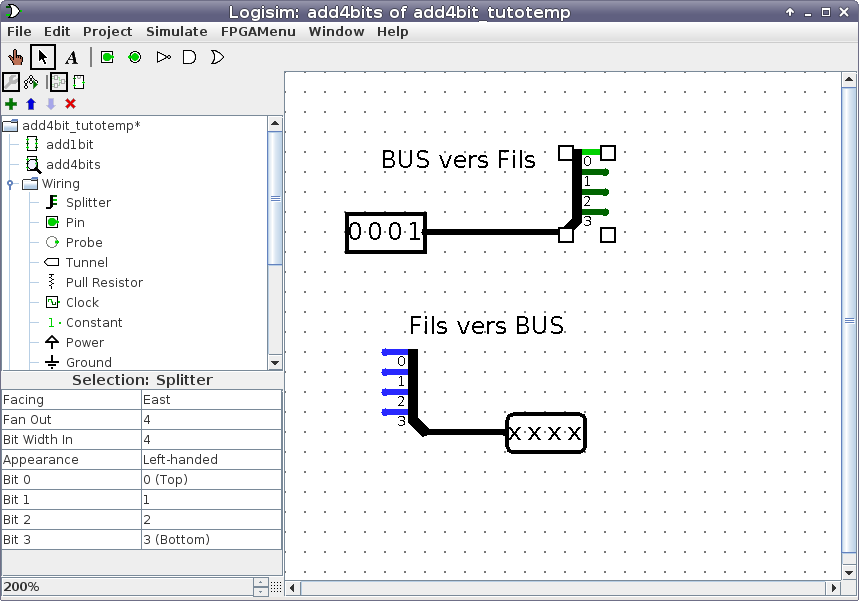
\includegraphics[width=350pt]{images/logisim_splitters.png}
\caption{\label{fig_splitter}Exemples splitters}
\end{center}
\end{figure}

Il faut définir les tailles d'entrées et de sorties du \texttt{splitter} via les attributs \texttt{Fan out} et
\texttt{Bit Width In}. Dans notre cas on définit les deux valeurs à 4.

Note: Le bit de poids faible est indexé à 0 en sortie du \texttt{splitter}.

\end{enumerate}

\section{Additionneur 4 bits}

Réalisez l'additionneur 4 bits en Figure~\ref{fig_add4bits}, puis vérifiez son bon fonctionnement en simulation.
Afin de faciliter la lecture des valeurs d'entrée/sortie, il est possible de changer le radix (binaire / octal / décimal) dans les options de la pin.
\begin{figure}[H]
\begin{center}
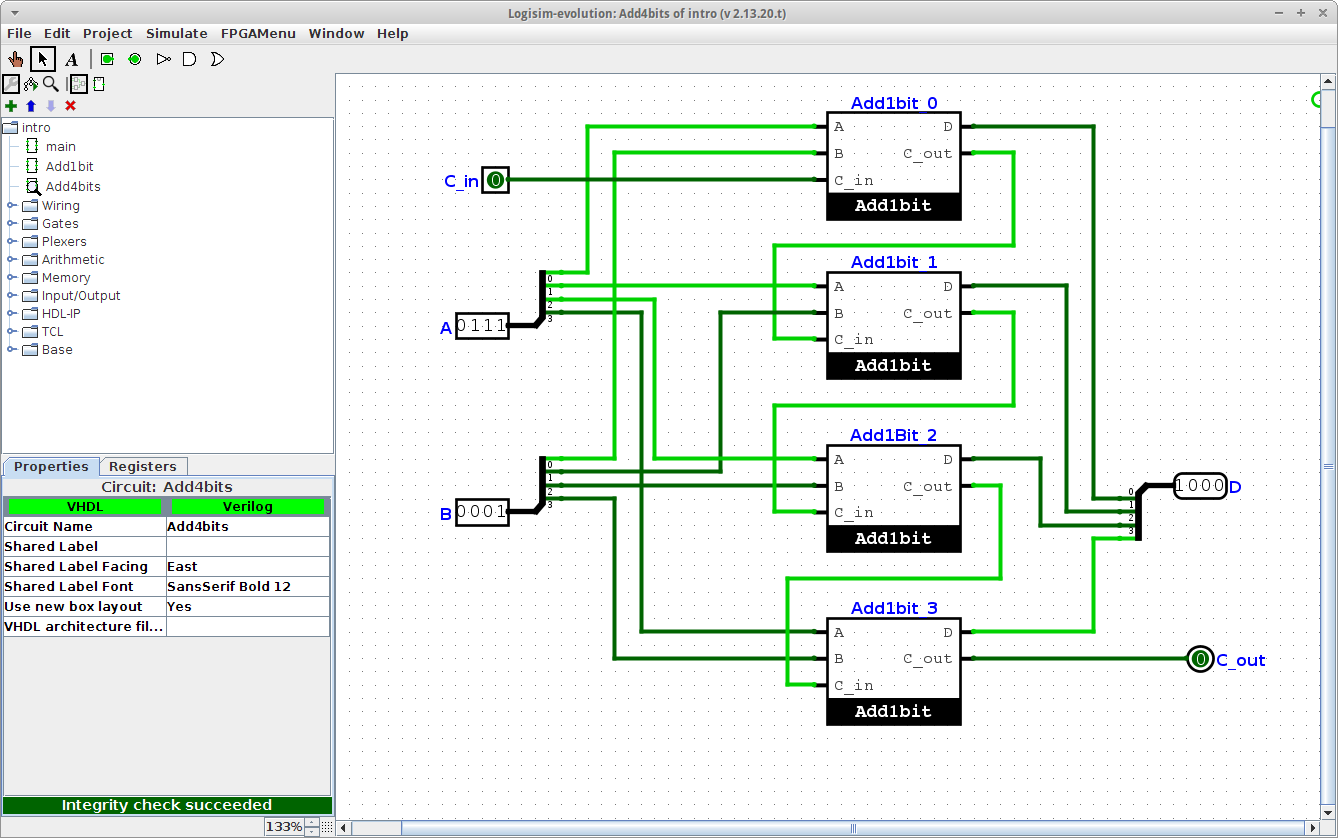
\includegraphics[width=385pt]{images/logisim_add4bits.png}
\caption{\label{fig_add4bits}Additionneur 4 bits}
\end{center}
\end{figure}

% =========================
%      Programmation
% =========================

\newpage
\section{Programmation de la carte MAX\_V avec la console}

\texttt{Logisim} permet de programmer directement la carte \texttt{MAX\_V}. Il faudra alors associer les
\texttt{Pin} en entrées à des boutons, et ceux des sorties à des LEDs.


\subsection{Connexion}
La carte \texttt{MAX\_V} et la \texttt{console} doivent être alimentées avec une alimentation 5 volts.
La programmation de la carte \texttt{MAX\_V} se fait via le module \texttt{USB-Blaster}.
Les éléments doivent être branchés comme sur la Figure~\ref{fig_connexion}.\\
\textbf{Matériel nécessaire:}
\begin{itemize}
\item Carte \texttt{MAX\_V},
\item Console,
\item Carte d'interface de la console,
\item Cable de liaison interface-\texttt{MAX\_V},
\item le module \texttt{USB-Blaster},
\item Cables d'alimentation.
\end{itemize}

\begin{figure}[H]
\begin{center}
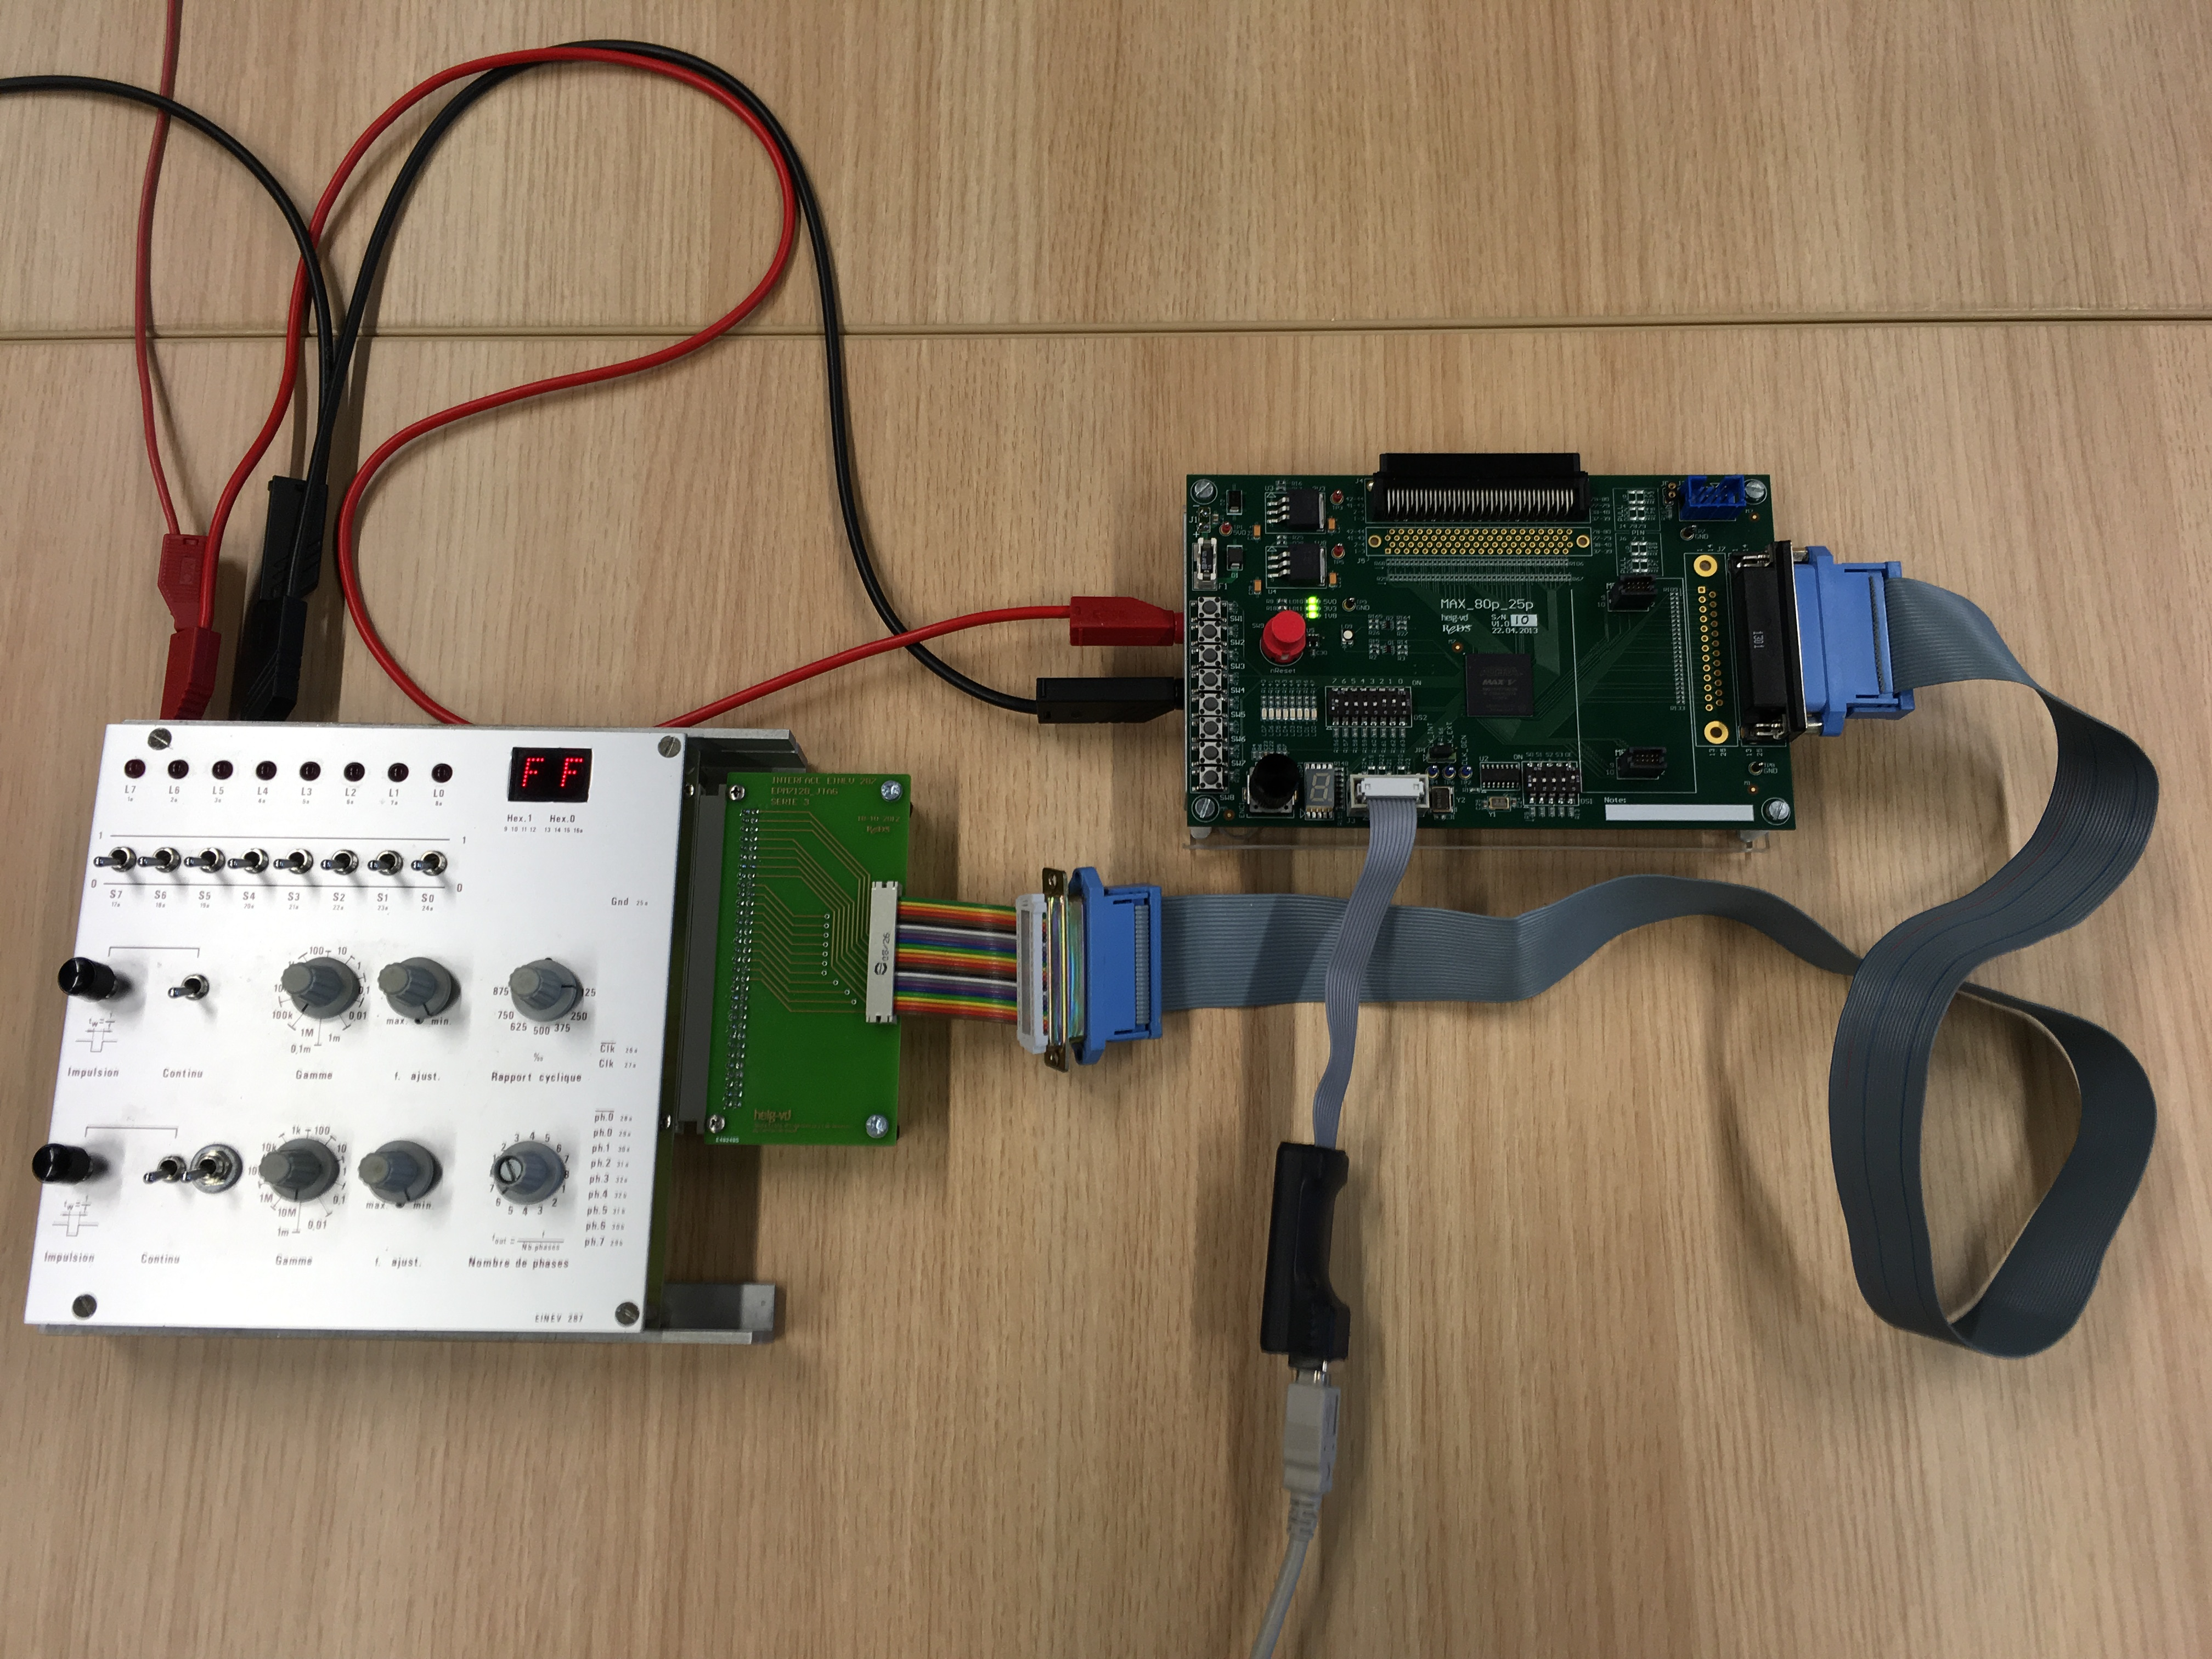
\includegraphics[width=0.85\linewidth]{images/MAXV_branchement.JPG}
\caption{\label{fig_connexion}Connexion de la carte MAX\_V avec la console}
\end{center}
\end{figure}

\subsection{Configuration}
\begin{enumerate}
\item Afin de pouvoir programmer la carte, il est nécessaire de nommer chaque entrée/sortie en leur affectant
l'attribut \texttt{Label}. On utilisera les termes \texttt{A}, \texttt{B} et \texttt{D} pour respectivement les deux bus
d'entrées et le bus de sorties. Les retenues seront nommées avec \texttt{C\_in} et \texttt{C\_out}.

Il faut aussi annoter tous les composants avec des identifiants uniques. Les quatre additionneurs 1 bits auront alors pour
label \texttt{add1bit\_X} ou \texttt{X} est un numéro unique.

\item On peut ensuite ouvrir l'interface de programmation via \texttt{FPGAMenu} -> \texttt{FPGA Commander}
comme sur la Figure~\ref{fig_FPGACommander}.

\begin{figure}[H]
\begin{center}
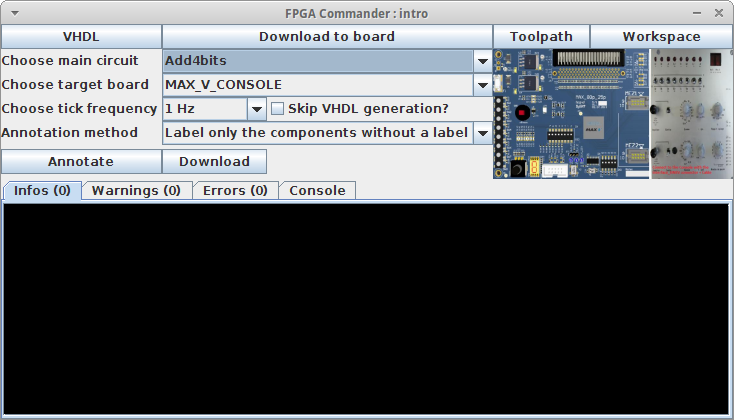
\includegraphics[scale=0.45]{images/logisim_fpgaCommander.png}
\caption{\label{fig_FPGACommander}FPGA Commander}
\end{center}
\end{figure}

\item Plusieurs paramètres doivent alors être définis:
\begin{itemize}
\item \textbf{Toolpath}: Il faut s'assurer qu'il pointe vers\\ \texttt{/opt/EDA/altera/13.0/quartus/bin}
\item \textbf{Workspace}: Il doit être défini vers \texttt{/home/redsuser/logisim\_workspace} %ou plutot c:\temp ?
\item \textbf{Choose main circuit}: Le circuit top level que nous voulons programmer. Dans notre cas c'est
\texttt{Add4bits}.
\item \textbf{Choose target board}: La carte que nous allons utiliser. Il faut choisir la carte du laboratoire
\texttt{MAX\_V\_CONSOLE}.
\item Les autres paramètres sont laissés à leur valeur par défaut.
\end{itemize}

\item Afin de programmer la carte \texttt{EPM 25p-25p}, Logisim va tout d'abord générer plusieurs fichiers
\texttt{.vhd}. Il faut pour cela cliquer sur \textbf{Annotate}, puis sur le bouton \textbf{Download}.
Tous les fichiers générés sont affichés dans l'onglet \texttt{Infos} du FPGA Commander.

\item Il faut ensuite associer les entrées/sorties de l'additionneur aux boutons et aux LEDs de la carte comme sur la
Figure~\ref{fig_mapping} et la Figure~\ref{fig_mapped}.

\begin{figure}[H]
\begin{center}
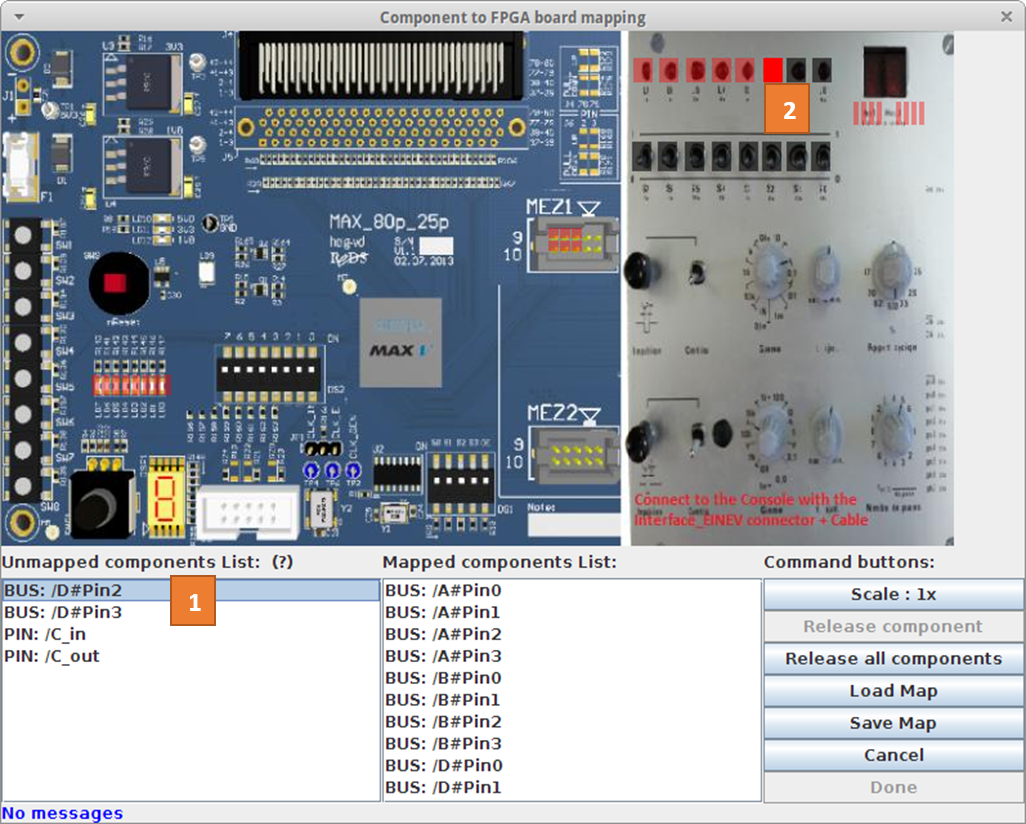
\includegraphics[scale=0.42]{images/logisim_mapping.png}
\caption{\label{fig_mapping}Console Board Mapping}
\end{center}
\end{figure}

\item Toutes les entrées/sorties que l'on a défini sont visibles dans le zone \textbf{Unmapped components list}. Si l'on veut
par exemple mettre le bit \texttt{0} de l'entrée \texttt{A} sur l'interrupteur tout en bas à droite de la carte, il faut
sélectionner \texttt{PIN: /A<0>}, puis cliquer sur l'interrupteur dans l'image. Si le mapping est possible, lorsque l'on
passe le curseur sur l'interrupteur, ce dernier devient rouge. Pour les pins C\_in et C\_out, il faut double-cliquer sur la ligne pour passer du type pin\_in/out au type switch/led.


\item Placez les éléments de la manière suivante \textbf{(cf Figure~\ref{fig_mapped})}:
\begin{itemize}
\item Les 4 bits de l'entrée \texttt{A} sur les 4 premiers switches (S0 à S3).
\item Les 4 bits de l'entrée \texttt{B} sur les 4 switches suivants (S4 à S7).
\item L'entrée \texttt{C\_in} sur le bouton poussoir (SW1).
\item Les 4 bits de la sortie \texttt{D} sur les 4 premières LEDs (L0 à L3).
\item La sortie \texttt{C\_out} sur la LED L7.\\
\end{itemize}
Une fois que toutes les entrées et sorties ont été définies, cliquez sur \texttt{Done} .

\begin{figure}[H]
\begin{center}
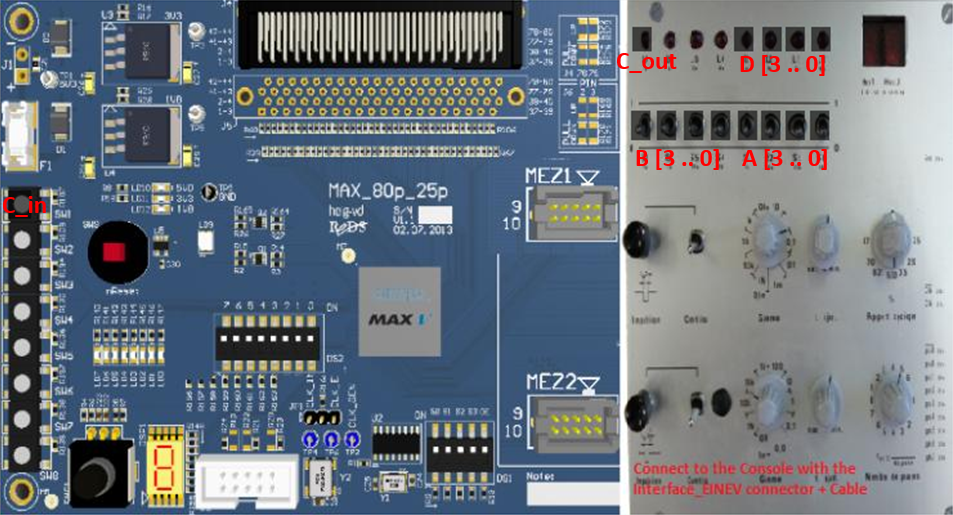
\includegraphics[width=350pt]{images/logisim_mapped.png}
\caption{\label{fig_mapped}Position des entrées/sorties}
\end{center}
\end{figure}

\item 
Après la compilation, une fenêtre apparaît pour demander à l'utilisateur si la carte est branchée. Brancher le connecteur usb du programmeur jtag au pc et le connecteur jtag à la carte. Allumer l'alimentation 5V puis cliquez sur \texttt{Yes, download}.\\
Une fois le téléchargement terminé, l'onglet Errors de la fenêtre de FPGA Commander indique si il y a eu des erreurs ou non.


\end{enumerate}


% =========================
%      Chronogramme
% =========================

\newpage
\section{Chronogramme}
En plus de pouvoir simuler en temps réel un schéma logique, Logisim peut représenter cette simulation sous la forme d'un
chronogramme. Si cette visualisation est peu adapté aux systèmes purement combinatoire, elle est très pratique dans le
cas des systèmes logiques séquentiels (utilisation d'horloges, ex: compteur, registres...).
Afin de vérifier le fonctionnement de l'additionneur en fonction du temps, il faut ajouter un compteur au circuit.

\begin{enumerate}
\item Créer un nouveau circuit dans le projet.
\item Insérer votre additionneur 4 bits dans le nouveau circuit.
\item Ajouter un compteur (le compteur se trouve dans les composants \texttt{Memory}). Editer le paramètre \texttt{Data bits}, sa valeur est 4.
\item Câbler le compteur et l'additionneur comme indiqué sur l'image suivante (les constantes se trouvent dans \texttt{Wiring}).
\end{enumerate}

Le circuit final doit ressembler à celui en Figure~\ref{fig_logisim_addcpt}.

\begin{figure}[H]
\begin{center}
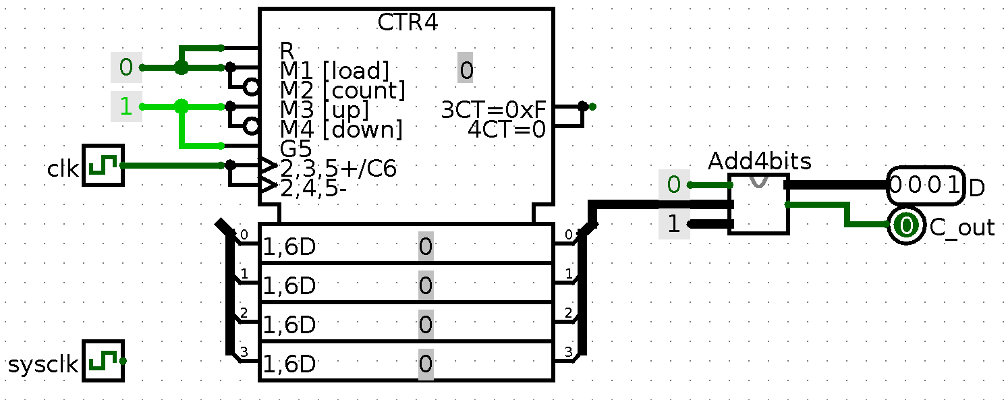
\includegraphics[width=450pt]{images/logisim_counter.png}
\caption{\label{fig_logisim_addcpt}Ajout du compteur}
\end{center}
\end{figure}


\subsection{Configuration du Chronogramme}
Pour pouvoir afficher le chronogramme, il faut définir une fréquence d'échantillonnage qui indiquera au système à quels
moments il doit afficher les valeurs de chaque signal. Cette fréquence doit être défini par une horloge d'échantillonnage
ajouté au circuit simulé, qui ne doit être reliée à aucun composant.

\subsubsection{Horloge d'échantillonnage}
Pour créer l'horloge d'échantillonnage il faut:
\begin{itemize}
\item Aller dans le liste de composant, prendre \texttt{Wiring -> clock} et l'ajouter au schéma.
\item Aller dans les attributs de cette horloge et la nommer \texttt{sysclk} (Attribut Label)
\item Assurez vous que les attributs \texttt{High Duration} et \texttt{Low duration} sont bien définis à un coup
d'horloge.
\item \textbf{Ne reliez cette horloge à aucun composants!}
\item Pour définir la fréquence de cette horloge: \texttt{Simulate -> Tick Frequency}. Prenez par exemple 4Hz.
\end{itemize}

\subsubsection{Ajout d'une horloge interne}
Placer une nouvelle horloge nommée \texttt{clk}. Logisim nécessite le nom \texttt{clk} pour le chronogramme, un autre nom ne convient pas.
L'horloge interne de votre système doit être plus lente que \texttt{sysclk}. Elle s'ajoute de la même façon que l'horloge
d'échantillonnage: \texttt{Wiring -> clock}.
Usuellement, on nome l'horloge de son système \texttt{clk}.

Le chronogramme va rechercher l'horloge dans le main circuit, pour changer votre circuit en main circuit,
il faut effectuer un clique droit sur votre composant (dans la liste des composants de la colonne de gauche) puis
sélectionner \texttt{Set As Main Circuit}.
Pour définir sa fréquence, il faudra modifier ses attributs afin de régler combien de ticks cette horloge nécessite
avant de changer d'état.  Par exemple si vous avez choisi une fréquence d'échantillonnage de 4Hz, mettez les attributs
\texttt{High duration} et \texttt{Low duration} de votre horloge à 4 ticks. Votre horloge changera alors d'état une fois
par seconde.

\subsubsection{Sélection des signaux}
Il faut ensuite définir quels signaux nous voulons afficher dans le chronogramme, comme en
Figure~\ref{fig_logisim_chrono_selection}.

\begin{figure}[H]
\begin{center}
    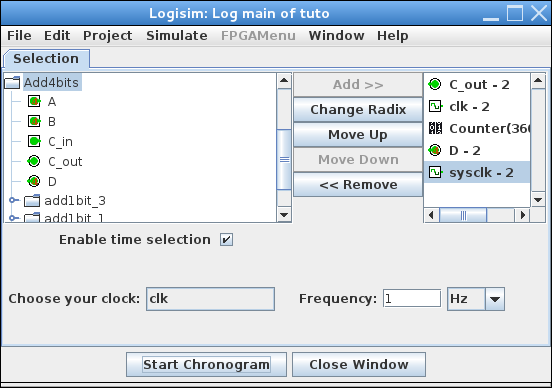
\includegraphics[scale=0.5]{images/chronoSelect.png}
\end{center}
\caption{\label{fig_logisim_chrono_selection}Sélection des signaux}
\end{figure}

\begin{itemize}
    \item Ouvrez le menu \texttt{Simulate} puis sélectionnez \texttt{Chronogram}.
        La liste des signaux disponibles apparait.
    \item Sélectionnez les signaux que vous voulez et cliquez sur \texttt{Add >>}
    \item Il est indispensable que l'horloge d'échantillonnage \texttt{sysclk} soit aussi ajoutée.
\end{itemize}

Il est possible (mais pas indispensable) d'afficher une base de temps, selon la fréquence d'un signal d'horloge. Il faut activer la case
\texttt{Enable time selection}, puis choisir l'horloge de votre système ainsi que sa fréquence.

Démarrez le chronogramme via le bouton \texttt{Start Chronogram}, puis organisez les fenêtres afin
d'être capable de voir à la fois le schéma et le chronogramme.
Le chronogramme final doit ressembler à celui en Figure~\ref{fig_logisim_chronogram}.

\begin{figure}[H]
\begin{center}
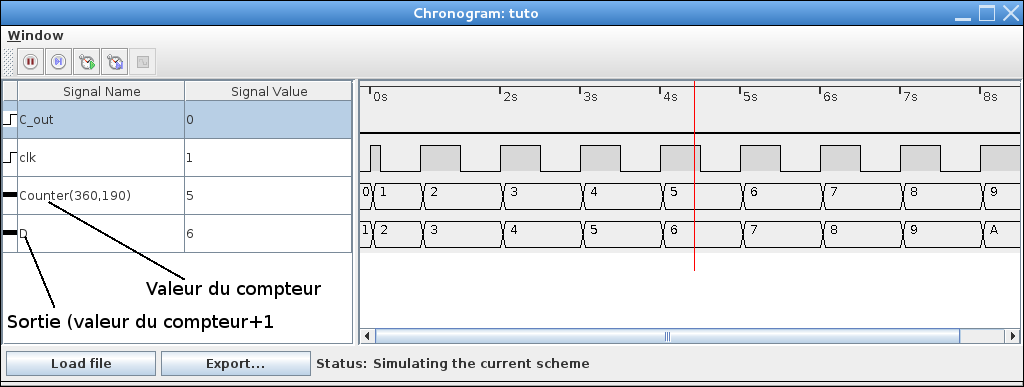
\includegraphics[width=450pt]{images/chrono.png}
\caption{\label{fig_logisim_chronogram}Chronogramme}
\end{center}
\end{figure}

\subsection{Utilisation du chronogramme}
A chaque changement d'état de l'horloge \texttt{sysclk}, le chronogramme se mettra à jour.

Il est aussi possible de démarrer et d'arrêter l'horloge: \texttt{Simulate -> Ticks Enabled} (Raccourci :
\texttt{Ctrl+k}). La touche \texttt{F2} permet d'avancer en mode pas à pas.

Contrôles du chronogramme:
\begin{itemize}
    \item Valeur à l'instant \texttt{t}: En cliquant sur un signal dans la partie droite du chronogramme, la valeur des
        données à cet instant sera affichée à coté du nom du signal.
    \item Scrollez avec la molette sur le chronogramme pour zoomer/dézoomer (focus sur la zone sélectionnée).
    \item Click droit sur un bus \texttt{->Format} pour changer son format d'affichage.
    \item Click droit sur un bus \texttt{->Expand} afficher chaque signal composant le bus.
\end{itemize}

\subsubsection{Sauvegarde et chargement}
Une fois la simulation terminée, vous pouvez exporter ce chronogramme dans un logFile via le bouton \texttt{Export}.
Créez un fichier \texttt{.txt} ou \texttt{.log} à l'emplacement souhaité.

Le chargement d'un de ces chronogrammes se fait via le bouton \texttt{Load External File}. Dans ce cas, le chronogramme
ne prend plus en compte les signaux du schéma courant. Il affiche simplement l'état des signaux tels qu'ils étaient lors
de l'export. Par ailleurs, si vous voulez utiliser le chronogramme uniquement pour visualiser un fichier préalablement
exporté, il faut simplement lancer le chronogramme avant de charger le fichier:
(\texttt{Simulate -> Chronogram -> Start Chronogram -> Load file}).


\end{document}
